\begin{frame}[fragile]{Visualização dos sinais no domínio do tempo}

    \begin{figure}
        \centering

        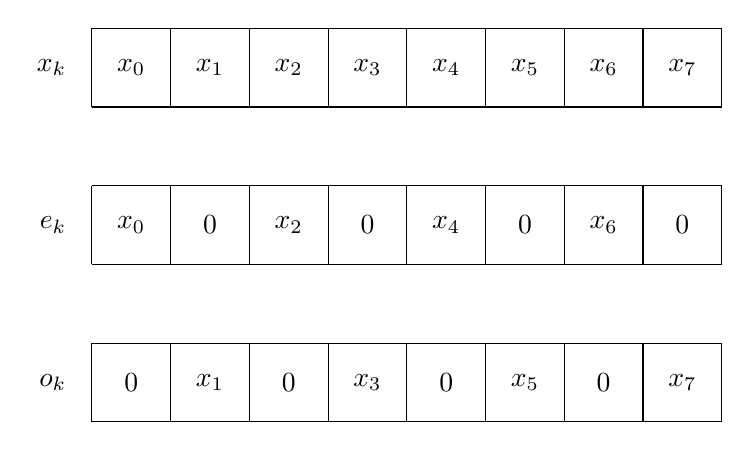
\begin{tikzpicture}
            \node[anchor=east] at (-0.2, 5.5) { $x_k$ };
            \draw (0, 5) grid (8, 6);

            \foreach \k in {0,...,7}
                \node at (\k + 0.5, 5.5) { $x_{\k}$ };

            \node[anchor=east] at (-0.2, 3.5) { $e_k$ };
            \draw (0, 3) grid (8, 4);

            \foreach \k in {0,...,3}
            {
                \pgfmathtruncatemacro{\label}{2*\k};
                \node at (2*\k + 0.5, 3.5) { $x_\label$ };
                \node at (2*\k + 1.5, 3.5) { $0$ };
            }

            \node[anchor=east] at (-0.2, 1.5) { $o_k$ };
            \draw (0, 1) grid (8, 2);

            \foreach \k in {0,...,3}
            {
                \pgfmathtruncatemacro{\label}{2*\k + 1};
                \node at (2*\k + 1.5, 1.5) { $x_\label$ };
                \node at (2*\k + 0.5, 1.5) { $0$ };
            }


        \end{tikzpicture}

    \end{figure}

\end{frame}

\begin{frame}[fragile]{Visualização das transformadas no domínio das frequências}

    \begin{figure}
        \centering

        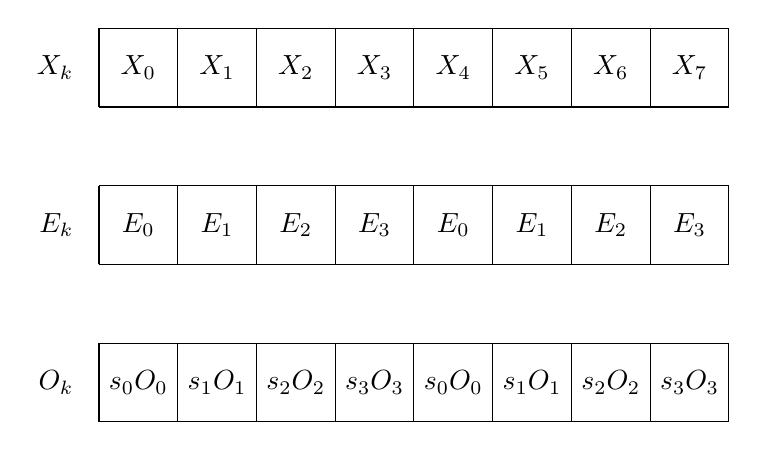
\begin{tikzpicture}
            \node[anchor=east] at (-0.2, 5.5) { $X_k$ };
            \draw (0, 5) grid (8, 6);

            \foreach \k in {0,...,7}
                \node at (\k + 0.5, 5.5) { $X_{\k}$ };

            \node[anchor=east] at (-0.2, 3.5) { $E_k$ };
            \draw (0, 3) grid (8, 4);

            \foreach \k in {0,...,3}
            {
                \pgfmathtruncatemacro{\label}{\k + 1 - 1};
                \node at (\k + 0.5, 3.5) { $E_\label$ };
                \node at (\k + 4.5, 3.5) { $E_\label$ };
            }

            \node[anchor=east] at (-0.2, 1.5) { $O_k$ };
            \draw (0, 1) grid (8, 2);

            \foreach \k in {0,...,3}
            {
                \pgfmathtruncatemacro{\label}{\k + 1 - 1};
                \node at (\k + 0.5, 1.5) { $s_\label O_\label$ };
                \node at (\k + 4.5, 1.5) { $s_\label O_\label$ };
            }


        \end{tikzpicture}

    \end{figure}

\end{frame}
